\section{Simulink model user guideline}

The dwelling model has been fist developed in Matlab/Simulink and convert to Python later on. In the Simulink model it is possible to define the dwelling characteristics, the dwelling use data and the climate data. With some of this information the model resistances and capacities are built on a Matlab script. The resistances and capacities values are used during the year energy simulation. 
In sections \ref{Dewellinginfo} to \ref{climatedata} the information provided to make the simulation is presented.

\subsection{Dwelling characteristics information}
\label{Dewellinginfo}
	
The dwelling characteristics taken into account in order to define the model resistances and capacities are presented in figure \ref{figure: Dwelling characteristic}. The ventilation rate n in ach (air changes per hour) is based on a mechanical ventilation rate of 150 m3/h for kitchen, toilet and bathroom) by regulations.

\begin{figure}[H]
	\centering
	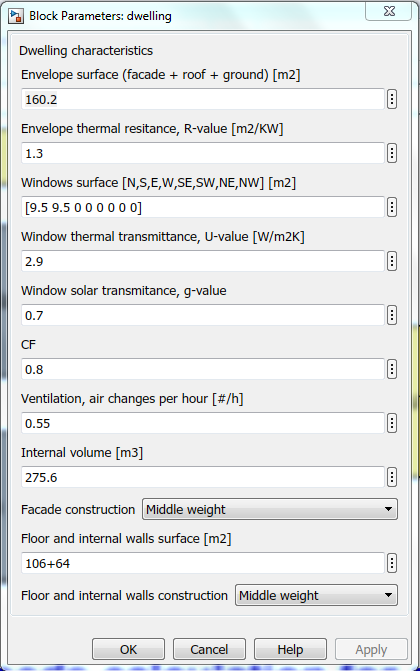
\includegraphics[width=0.8\columnwidth]{Pictures/dwelling characteristic model information.png}
	\caption[Short title]{Dwelling characteristic model information}
	\label{figure: Dwelling characteristic}
\end{figure}
\newpage
\subsection{Dwelling use data}
\label{Dwelling use data}

The dwelling use data define the schedule to be used to calculate the dwelling internal heat and the thermostat set-points. The thermostat signal is communicated to the heat pump model. The information use to define the dwelling use is presented in figure \ref{figure:Dwelling info}


\begin{figure}[H]
	\centering
	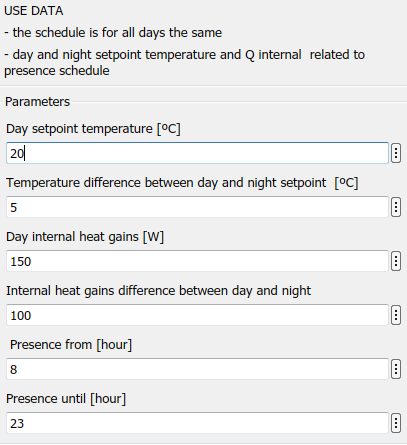
\includegraphics[width=0.8\columnwidth]{Pictures/Dwelling use model information.png}
	\caption[Short title]{Dwelling use model information}
	\label{figure:Dwelling info}
\end{figure}
\newpage
\subsection{Climate data}
\label{climatedata}
The hourly data about the outdoor temperature and the solar radiation is extracted from the NEN5060:2018 norm. This norm defines a typical meteorological year using the Finkelstein-Schafer statistical method with the climate data of 20 years period (1996-2015). The meteorological data used by the norm is updated once every 5 years.  

The typical meteorological year data is the one to be used when calculating the typical energy use of the heating installation. The NEN norm offers also three other hourly climate data sets, each one with a different perceptual deviation from the typical meteorological year: 1\%, 3\% and 5\%. These data sets are to be used when analysing the response of the heating installation under more extreme climate conditions. This is usually done for design installation purposes. The total energy use calculated with these other data sets will not give a reliable value for calculating the typical energy use.  In figure \ref{figure Climate data selection} it is shown that is it possible to choose between the four different NEN climate data sets. 

\begin{figure}[H]
	\centering
	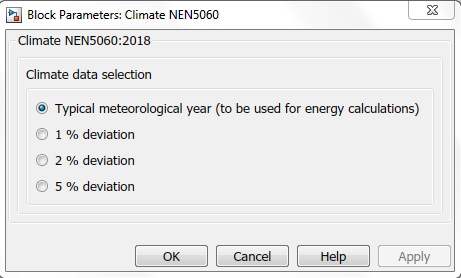
\includegraphics[width=0.8\columnwidth]{Pictures/climate data selection.png}
	\caption[Short title]{Climate data selection}
	\label{figure Climate data selection}
\end{figure}

In a pre-process the global incident radiant is calculated for North, South, East, West, North-West, North-East, South-West and South-East orientations of the façade in Matlab. The model from Perez is applied for the exchange. In this model the irradiation is split into a direct and diffuse terms.
\newpage
